\documentclass[11pt]{article}
\usepackage{fancyhdr}
\usepackage{tocloft}
\usepackage{graphicx}
\usepackage{calc}
\usepackage{amssymb}
\usepackage{color}
\usepackage[sc]{mathpazo}
\usepackage{url}
\usepackage{ifpdf}
\usepackage{bbding}
\usepackage{caption}
\usepackage{framed}
\usepackage{xcolor}
\usepackage{float}
\usepackage{wrapfig}
\usepackage{sidecap}
\linespread{1.0}
\oddsidemargin=0pt
\evensidemargin=0pt
\textwidth=6.5in
\topmargin=0pt
\headheight=0pt
\headsep=0pt
\textheight=9in
\setlength{\parindent}{0.25cm}
\newcommand\secfont{\fontfamily{cmss}\selectfont}%\textwidth 5.5truein
\newcommand\pifheading[1]{\noindent{\secfont\textbf{#1}:}}
\newcommand\yr{2016}
\def\lo{
\mathrel{\raise.3ex\hbox{$<$}\mkern-14mu\lower0.6ex\hbox{$\sim$}}
}
\def\hi{
\mathrel{\raise.3ex\hbox{$>$}\mkern-14mu\lower0.6ex\hbox{$\sim$}}
}

\textwidth = 6.5 in
\textheight = 9 in
\oddsidemargin = -0.00 in
\evensidemargin = +0.05 in
\topmargin = 0 in
\headheight = 0.0 in
\headsep = 0.0 in
\parskip = 0.05in

\newcommand\registered{{\ooalign{\hfil\raise .00ex\hbox{\scriptsize R}\hfil\crcr\mathhexbox20D}}}

%% Define a new 'leo' style for the package that will use a smaller font.
\makeatletter
\def\url@leostyle{%
  \@ifundefined{selectfont}{\def\UrlFont{\sf}}{\def\UrlFont{\small\ttfamily}}}
\makeatother
%% Now actually use the newly defined style.
\urlstyle{leostyle}
\newcommand\checkme[1]{\textcolor{blue}{\textbf{#1}}}
\newcounter{hours}\newcounter{minutes}
\newcommand\printtime{\setcounter{hours}{\time/60}\setcounter{minutes}{\time - \value{hours}*60}\thehours :\theminutes}
\newenvironment{packed_item}{
\begin{itemize}
 \setlength{\itemsep}{1pt}
 \setlength{\parskip}{0pt}
 \setlength{\parsep}{0pt}
}{\end{itemize}}

\newenvironment{packed_enum}{
\begin{enumerate}
 \setlength{\itemsep}{1pt}
 \setlength{\parskip}{0pt}
 \setlength{\parsep}{0pt}
}{\end{enumerate}}

\newenvironment{box_list}{
\begin{itemize}
 \setlength{\itemsep}{3pt}
 \setlength{\parskip}{0pt}
 \setlength{\parsep}{0pt}
}{\end{itemize}}

\newenvironment{packed_list}{
\begin{list}{\labelitemi}{\leftmargin=1em}
 \setlength{\itemsep}{3pt}
 \setlength{\parskip}{0pt}
 \setlength{\parsep}{0pt}
}{\end{list}}

\renewenvironment{quote}{%
  \list{}{%
    \leftmargin10pt   % this is the adjusting screw
    \rightmargin\leftmargin
  }
  \item\relax
}
{\endlist}

% definition of a new float type (refer to the caption package documentation)
\DeclareCaptionType{boxcaption}[Box]
\captionsetup[boxcaption]{position=top,labelfont=bf}

% definition of a shaded-like environment (see framed.sty)
\newenvironment{shadedframe}
  {\def\FrameCommand{\setlength\fboxsep{10pt}\fcolorbox{black}{shadecolor}}%
    \MakeFramed {\advance\hsize-\width \FrameRestore}}%
{\endMakeFramed}

\newenvironment{shadedbox}{%
  \def\FrameCommand{\colorbox{shadecolor}}%
  \MakeFramed {\FrameRestore}}%
 {\endMakeFramed}

% main environment
% syntax: \begin{myenv}{placement-specifiers}{color}{width}...\end{myenv}
\newenvironment{boxenv}[3]
  {\colorlet{shadecolor}{#2}%
    \begin{boxcaption}[#1]%
    \noindent\begin{minipage}{#3}
      \begin{shadedframe}
      }
  {\end{shadedframe}\end{minipage}\end{boxcaption}}

 % TOC
\usepackage{enumerate}
\begin{document}


\begin{figure}
  
\includegraphics[width=\linewidth/3]{title}
  \label{fig:title}
\end{figure}


\title{Lab Report 7: Operational Amplifiers}


\author{Yuezhe Yao}

%\institute{Syracuse University}



\maketitle

\begin{abstract}
In this lab, we explored the basic properties of op amps in such feedback circuits, designed and characterized some of the most widely used op-amp circuits, including ones for amplification, signal addition and subtraction, and signal integration and differentiation.  
\end{abstract}

\medskip

\begingroup
\let\clearpage\relax
\tableofcontents
\endgroup

\medskip
\medskip

\section{Learning Objectives}

To learn and commit to memory the Golden Rules of op amp operation.

To develop experience in op amp circuit design and operation; and to become familiar with some basic op amp circuits and terminology.

To gain additional experience constructing circuits on the 503 proto-typing board.

To develop an appreciation for the importance of op amps in general.

\section{Activity I - The Op-Amp Follower}


\begin{figure}[H]
 \begin{center}
  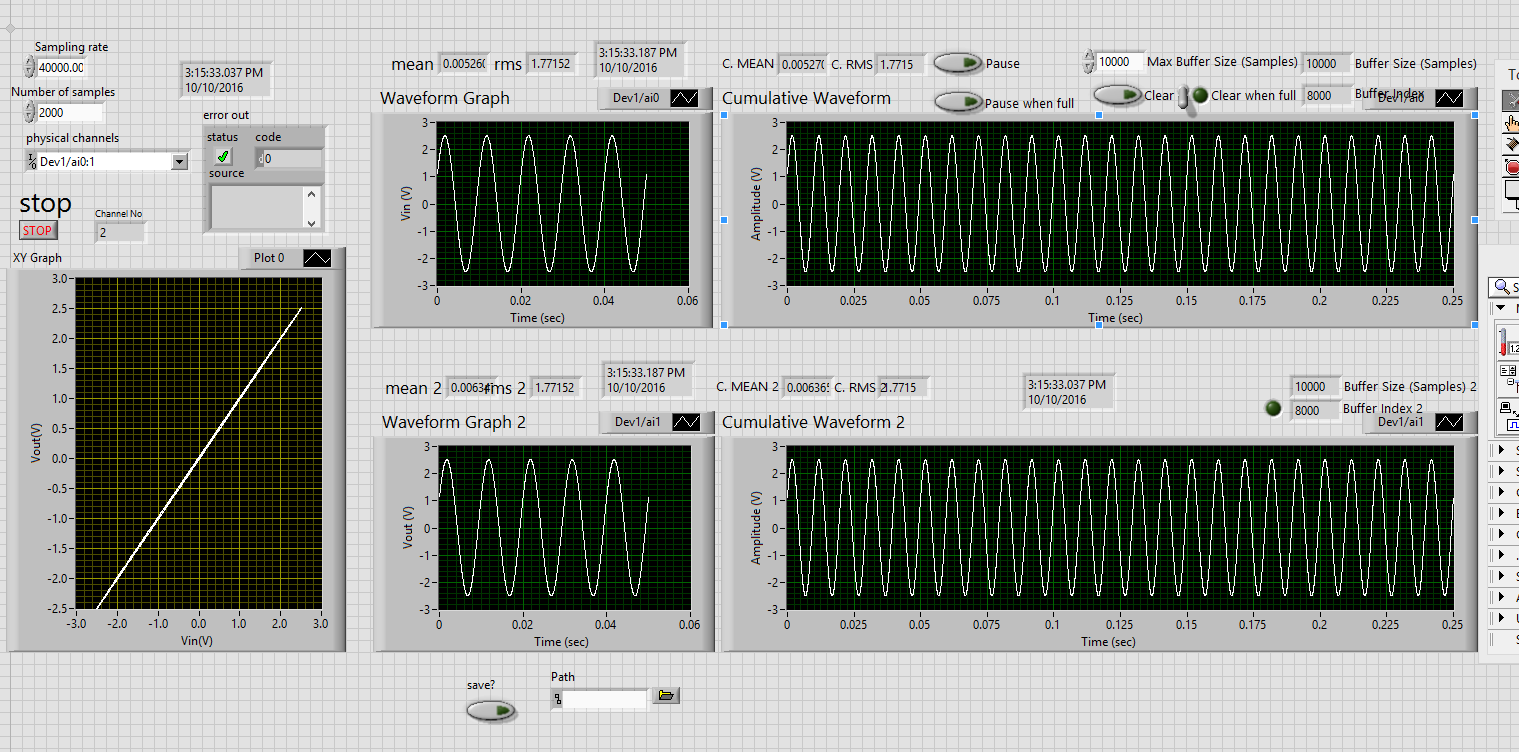
\includegraphics[width=\linewidth/1]{act1a100Hz}
  \caption{The front panel of the oscilloscope VI.}
  \label{fig:act1a100Hz}
 \end{center}
\end{figure}

From figure 1 we can see that the output signal is equal to the input signal, which is consistent with the function of the op-amp follower.

Due to the golden rules, the signal inputs draw no current, so the input impedance is very large, like $10^{12} \Omega$. And the output impedance is very small (close to zero), we used the following method to measure the output impedance.

First, we measured $V_{\mathrm{open}}=5.03V$, then add a larger resistor between the $V_{\mathrm{output}}$ and the ground, (to guarantee that the current won't saturate, and got the $V_{\mathrm{load}}=4.98V$ and $R_{\mathrm{load}}=192.4 \Omega$, so the current is $I=4.98/192.4=0.0259A$, and the output impedance is $R=\Delta V/I=(5.03-4.98)/0.0259=1.92 \Omega$, which is consistent with what we expect.

The bandwidth is $2*10^6 $Hz. We set the $V_{in}=V_{\mathrm{pp}}$ as 0.2V, then find the frequency when output signal $V_{\mathrm{out}}=V_{in}/\sqrt{2}=0.1414V$, which is 2 million Hz.
For this activity we can only use the Tektronix scopes to do this, we can't use the DAQmx and the VI because the sampling rate can not be set high enough for 2 million Hz input signal now.


\section{Activity II - The Inverting Amplifier}


\begin{figure}[H]
 \begin{center}
  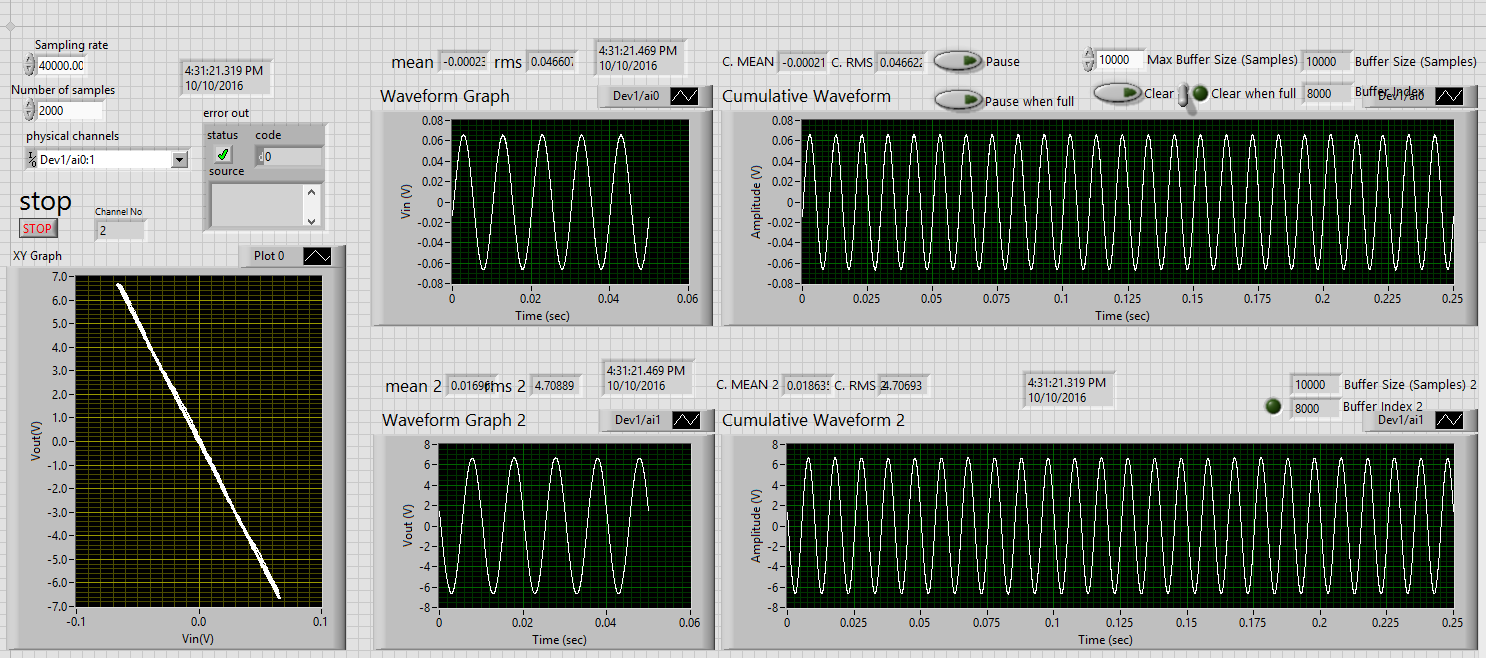
\includegraphics[width=\linewidth/1]{act2100Hz}
  \caption{The the front panel of the oscilloscope VI.}
  \label{fig:act2100Hz}
 \end{center}
\end{figure}

By the golden rule, The output of the op-amp attempts to do whatever is necessary to make the voltage difference between the inputs zero, and the signal inputs draw no current, so in this inverting amplifier
$V_{\mathrm{+}}=V_{\mathrm{-}}$, and because $V_{\mathrm{-}}$ is grounded, so $V_{\mathrm{+}}$ is like grounded also, which is called "virtual ground", so that $V_{\mathrm{in}}/R_{\mathrm{1}}=-V_{\mathrm{out}}/R_{\mathrm{2}}$, which is $V_{\mathrm{out}}=-{R_{\mathrm{2}} \over{R_{\mathrm{1}}}}V_{\mathrm{in}}$, and the input impedance is $\Delta V/ \Delta I={{4V-3.5V}\over{0.00171A-0.001665A}}=11111.11\Omega$


First we chose $R_{\mathrm{1}}=100 \Omega$ and $R_{\mathrm{2}}=10k \Omega$, so that the gain is $Gain={R_{\mathrm{2}} \over{R_{\mathrm{1}}}}={10000 \over100}=100$. And we the bandwidth we got is 150kHz, by using the same way in activity I. Because the gain is 100, so the bandwidth in Activity I with the follower should be 100 times of the bandwidth here, which is consistent.

\begin{figure}[H]
 \begin{center}
  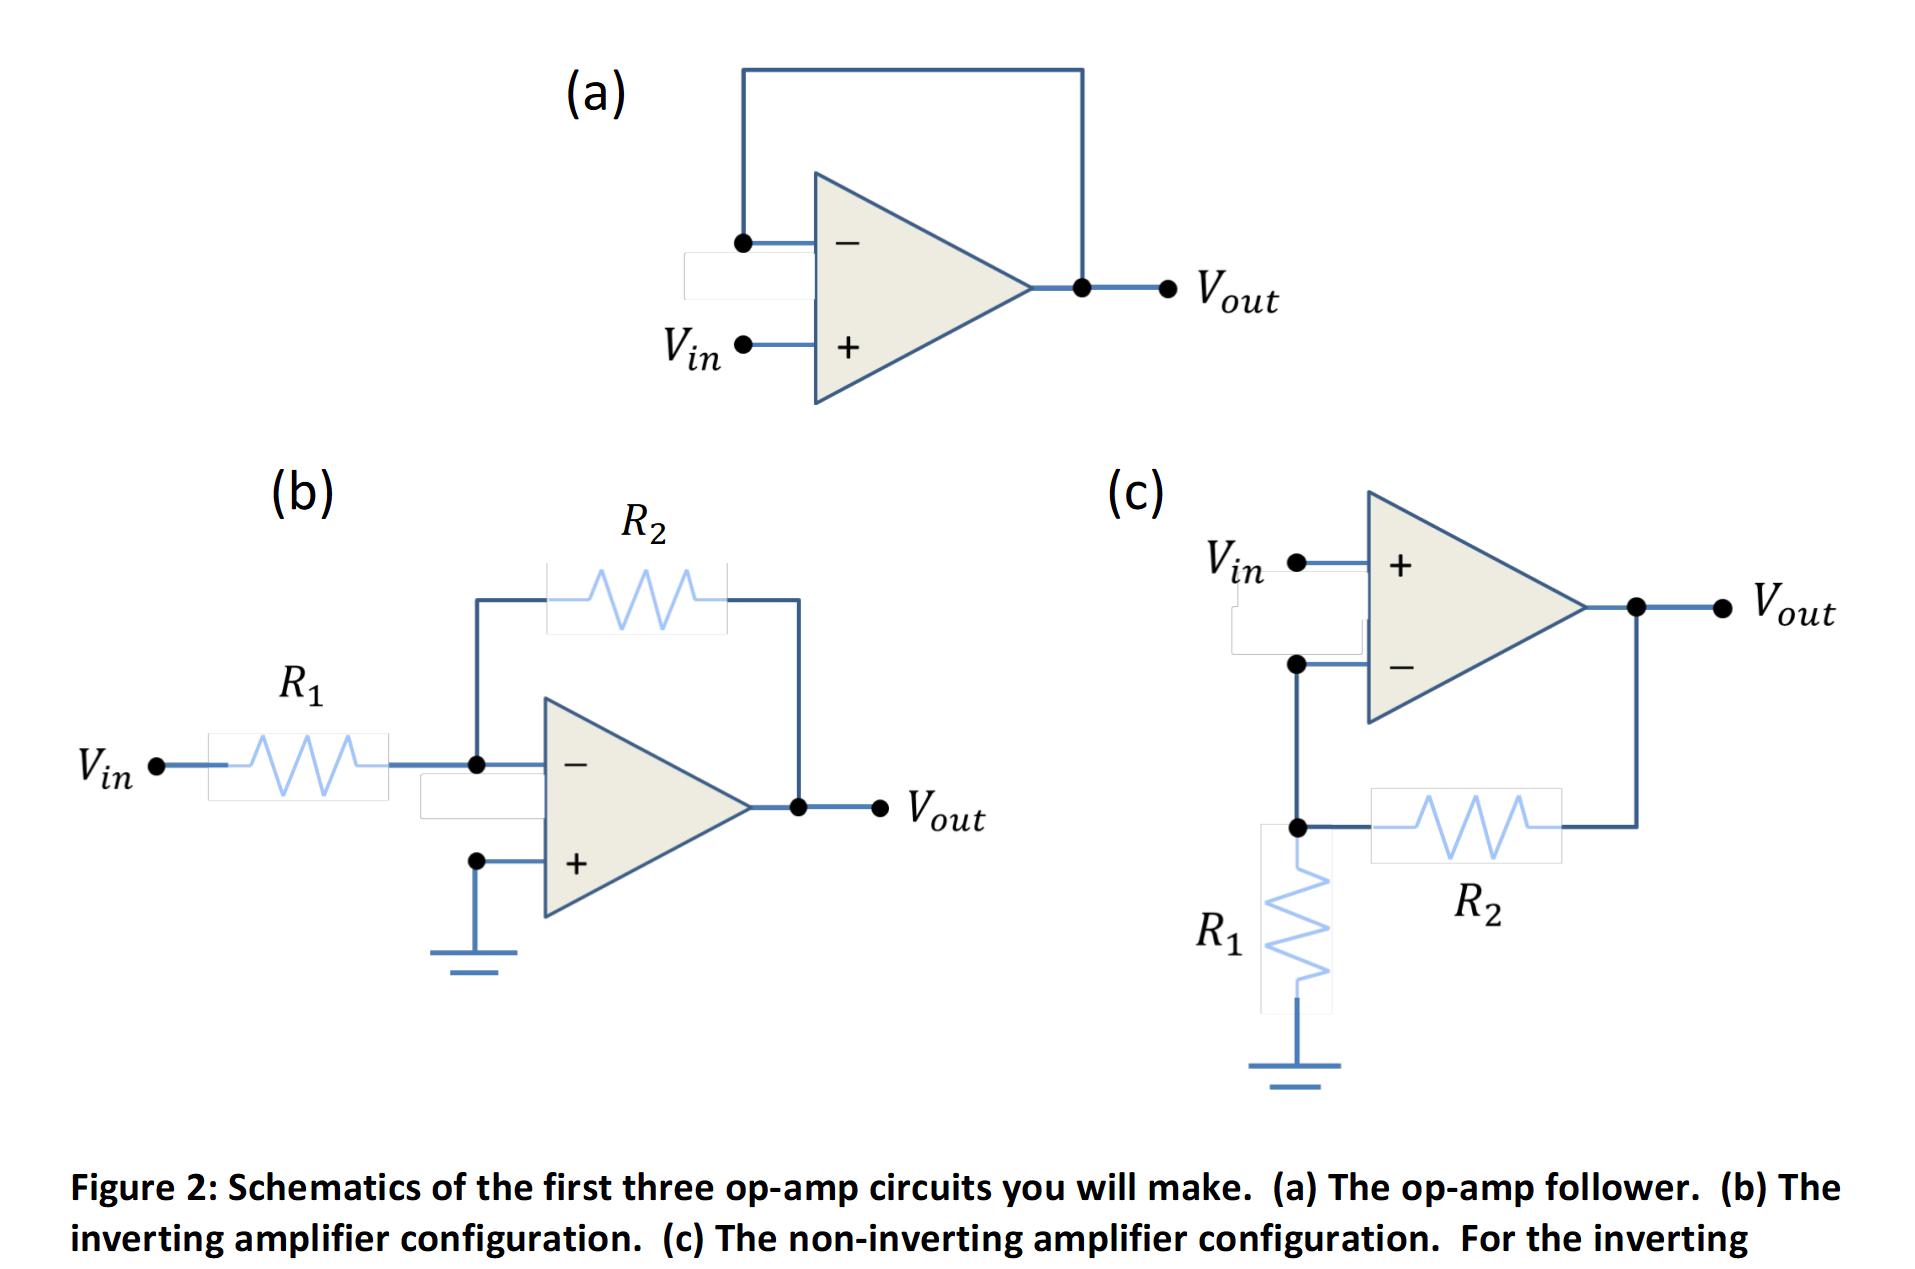
\includegraphics[width=\linewidth/2]{amplifier}
  \caption{}
  \label{fig:amplfier}
 \end{center}
\end{figure}

\section{Activity III - The Non-Inverting Amplifier}


\begin{figure}[H]
 \begin{center}
  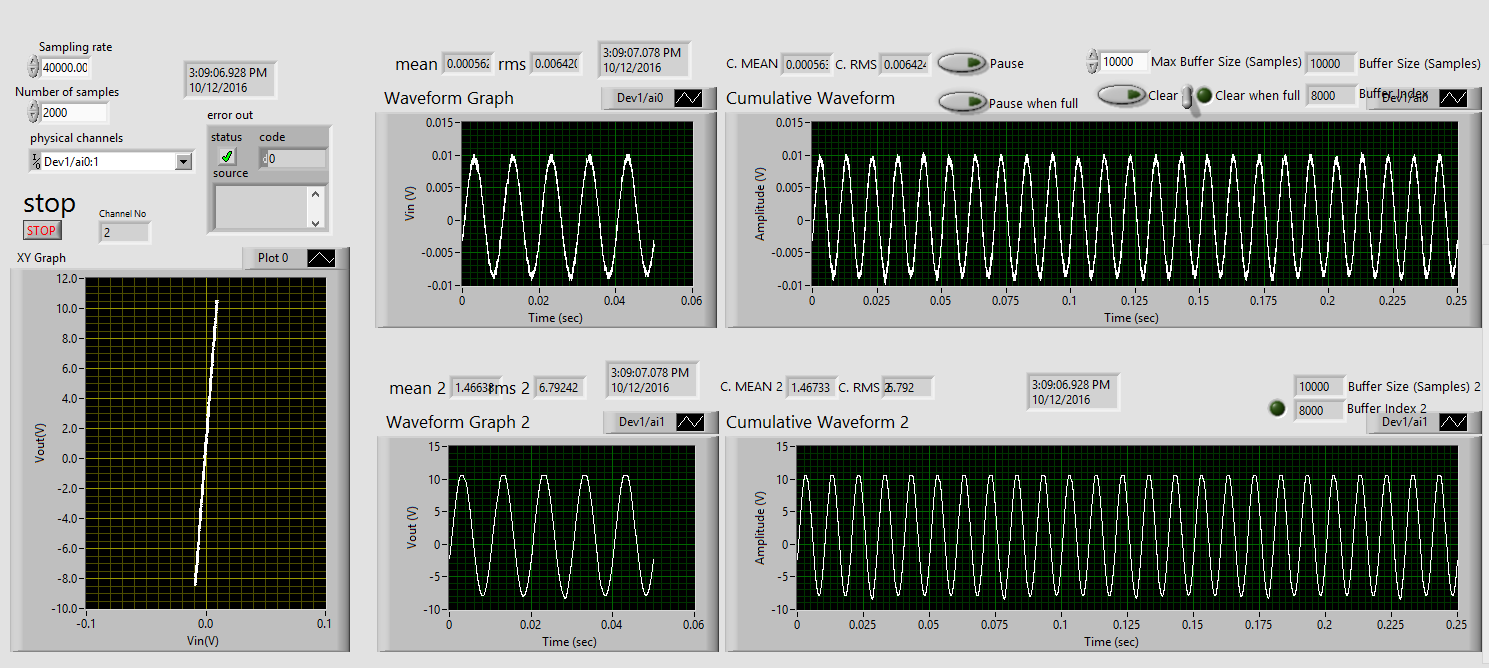
\includegraphics[width=\linewidth/1]{act3_1000times}
  \caption{The front panel of the VI for gain of 1000.}
  \label{fig:act3_1000times}
 \end{center}
\end{figure}

\begin{figure}[H]
 \begin{center}
  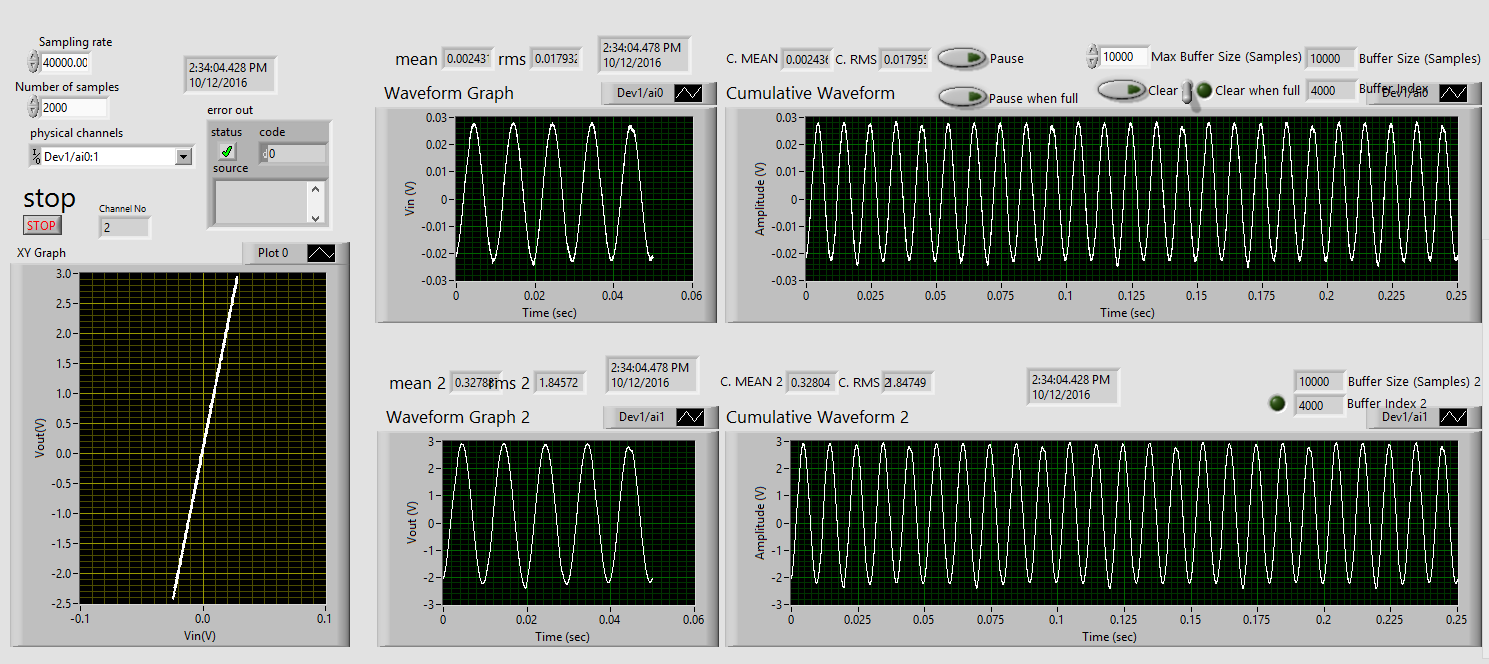
\includegraphics[width=\linewidth/1]{act3_100times}
  \caption{The front panel of the VI for gain of 100.}
  \label{fig:act3_100times}
 \end{center}
\end{figure}

For non-inverting amplifier,

$V_{\mathrm{in}}=V_{\mathrm{+}}=V_{\mathrm{-}}$

$\Rightarrow I_{\mathrm {R_{1}}}=V_{\mathrm{-}}/R_{\mathrm {1}}$ 

$\Rightarrow {\displaystyle V_{\mathrm{out}}=V_{\mathrm{in}}+I_{\mathrm {R_{1}}}R_{2}=V_{\mathrm{in}}\left(1+{\frac {R_{2}}{R_{1}}}\right)} $

And because "The signal inputs draw no current", so the input impedance=$V_{in}/I_{in}$=infinity.

We chose $R_{2}=10k \Omega$ and $R_{1}=100 \Omega$ to get the gain of 100, and we chose $R_{2}=100k \Omega$ and $R_{1}=100 \Omega$ to get the gain of 1000. And from the screen shots, we can see that the results are consistent with what we expect.

The measured bandwidth for gain of 100 is 62 kHz, and for gain of 1000 is 5 kHz. And we found that these results make sense because in activity I when the gain is 1, the magnitude of the bandwidth is $\sim10^6$Hz, and now when gain is 100, the magnitude is $\sim10^4$Hz, and the magnitude is $\sim10^3$Hz for the gain of 1000.

\vbox{}

\begin{figure}[H]
 \begin{center}
  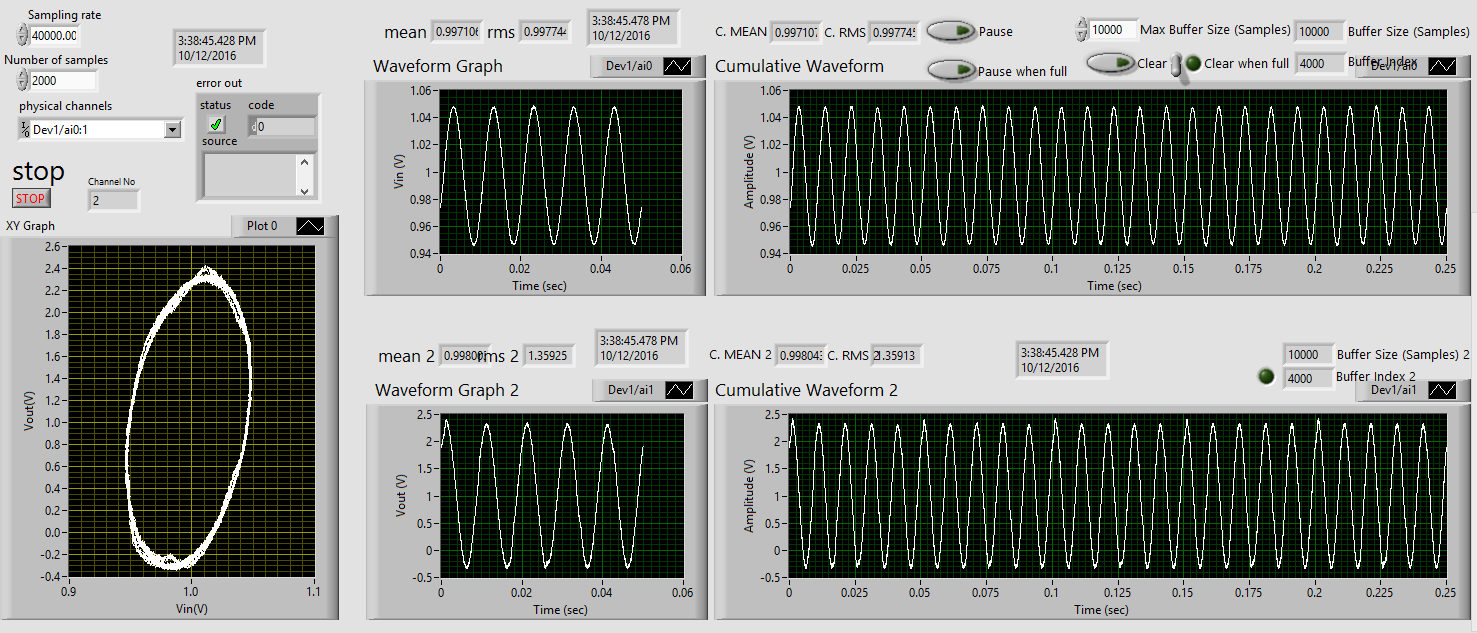
\includegraphics[width=\linewidth/1]{act3_4}
  \caption{The front panel of the VI with a capacitor and DC offset of 1V.}
  \label{fig:act3_4}
 \end{center}
\end{figure}

The way to "roll off" the gain to unity at DC is to insert a capacitor in series with $R_{1}$. And we chose the capacitor of $4.3 \mu F$ and set the DC offset as 1V. And from the picture above we can see it works, the DC offset was not amplified.

so use the impedance $R_{1}+{1 \over{i\omega C}}$ instead of $R_{1}$, the transform function

$TF\ ={V_{out}\over{V_{in}}}$

$\qquad = {{{R_{2}+(R+{1 \over{i\omega C}})}}\over{{R+{1\over{i\omega C}}}}}$

$\qquad = 1+ {{{R_{2}}}\over{{R+{1\over{i\omega C}}}}}$

$\qquad = {{{1+i\omega C(R_{2}+R)}}\over{{1+{i\omega CR}}}}$

\begin{figure}[H]
 \begin{center}
  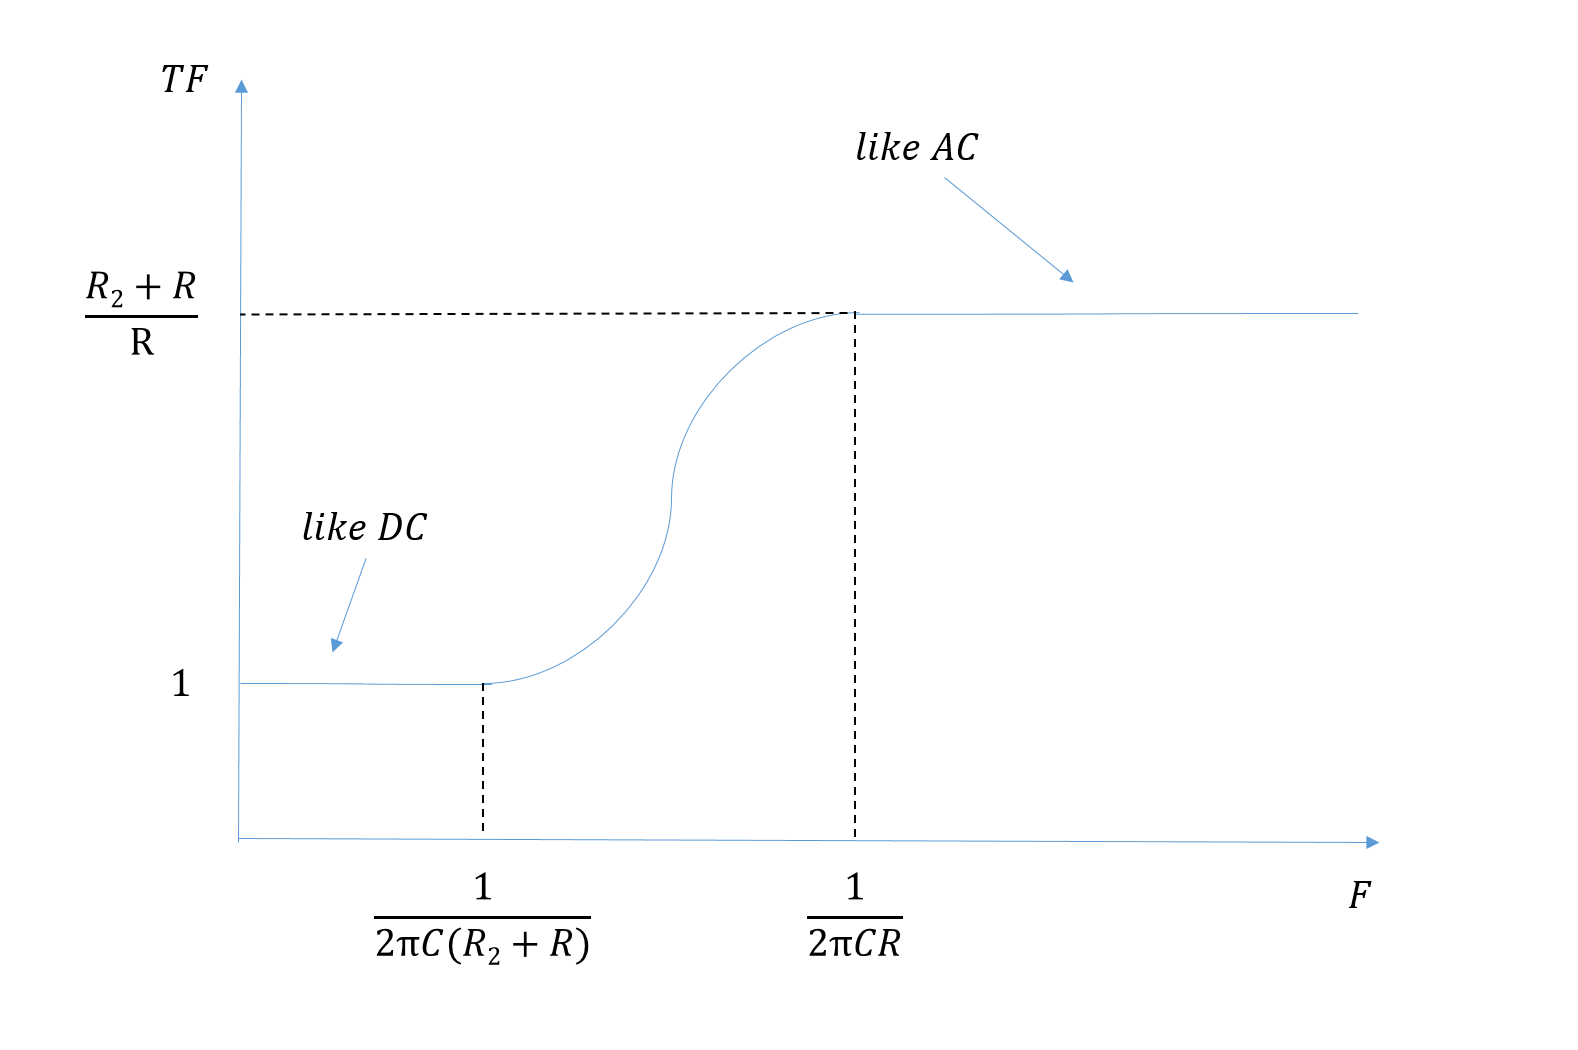
\includegraphics[width=\linewidth/1]{act3_4b}
  \caption{The transform function with a capacitor.}
  \label{fig:act3_4b}
 \end{center}
\end{figure}


\section{Activity IV - The Difference Amplifier}

\begin{figure}[H]
 \begin{center}
  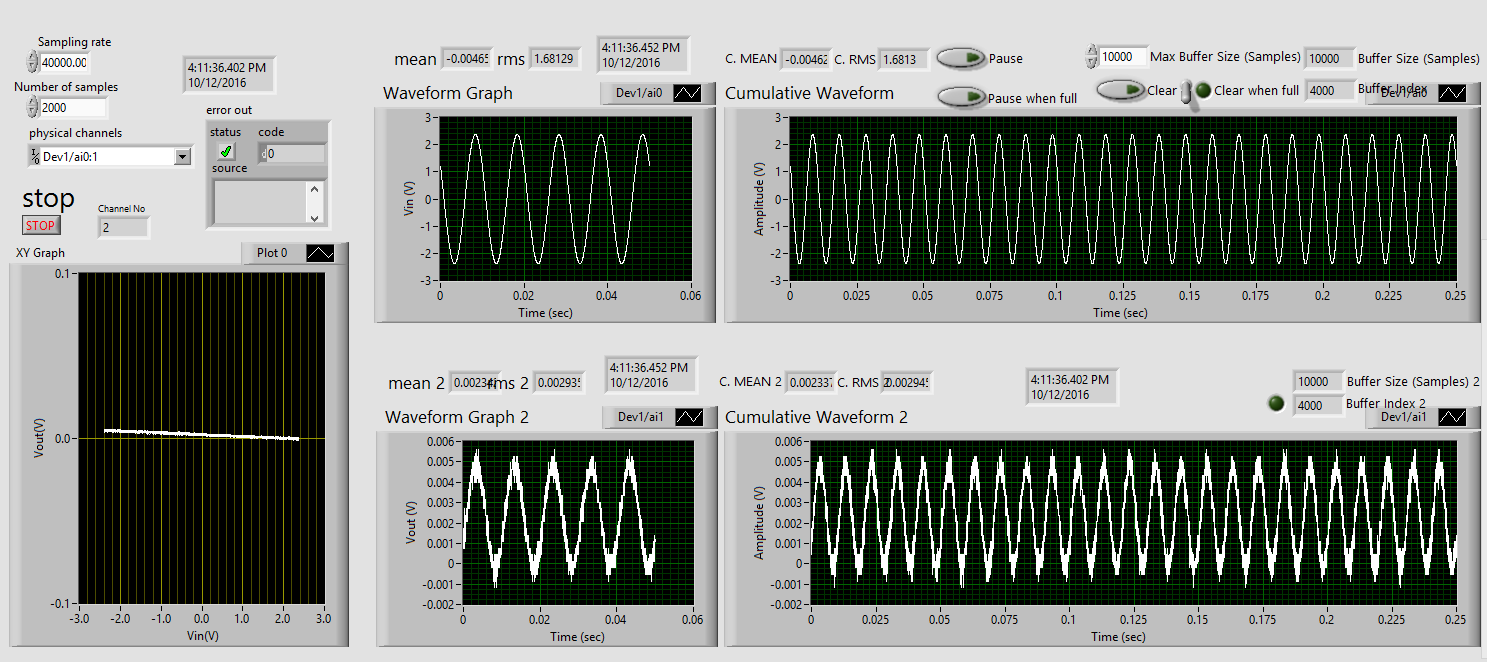
\includegraphics[width=\linewidth/1]{act4AC_V1eqV2}
  \caption{The front panel the VI when $V_{1}=V_{2}$.}
  \label{fig:act4AC_V1eqV2}
 \end{center}
\end{figure}

As shown in the picture above, we set $V_{2}=V_{1}=V_{in}$, so you can see that in our plot $V_{out}=V_{2}-V_{1} \approx 0$, which is consistent with what we expect. And the following shows the derivation of the operation of the ideal difference amplifier.

$I_{1}={V_{1}-V_{-}\over R_{1}}$

$I_{2}={V_{2}-V_{+}\over R_{2}}$

$I_{f}={V_{-}-V_{out}\over R_{f}}$

$V_{+}=V_{-}$ (Because of the golden rule)

$V_{+}=V_{2}({R_{3}\over R_{2}+R_{3}})$

if $V_{2}=0$, then $V_{out-}=-V_{1}({R_{3}\over R_{1}})$

if $V_{1}=0$, then $V_{out+}=V_{2}({R_{3}\over R_{2}+R_{3}})({R_{1}+R_{3}\over R_{1}})$

$V_{out}=V_{out-}+V_{out+}=-V_{1}({R_{3}\over R_{1}})+V_{2}({R_{3}\over R_{2}+R_{3}})({R_{1}+R_{3}\over R_{1}})$

so, if $R_{1}=R_{2}=R_{3}=R_{f}$

then $V_{out}=V_{2}-V_{1}$

And our observations are different from the case of an ideal difference amplifier, the $V_{out}\over V_{in}$ plot in frequency domain shows that there is a 1/300 rejection in DC when the frequency is low. And when it goes to the high frequency, the rejection degenerate. And there is a trough when the frequency is around 15MHz because of the phase shift. The following picture shows what we observed.

\begin{figure}[H]
 \begin{center}
  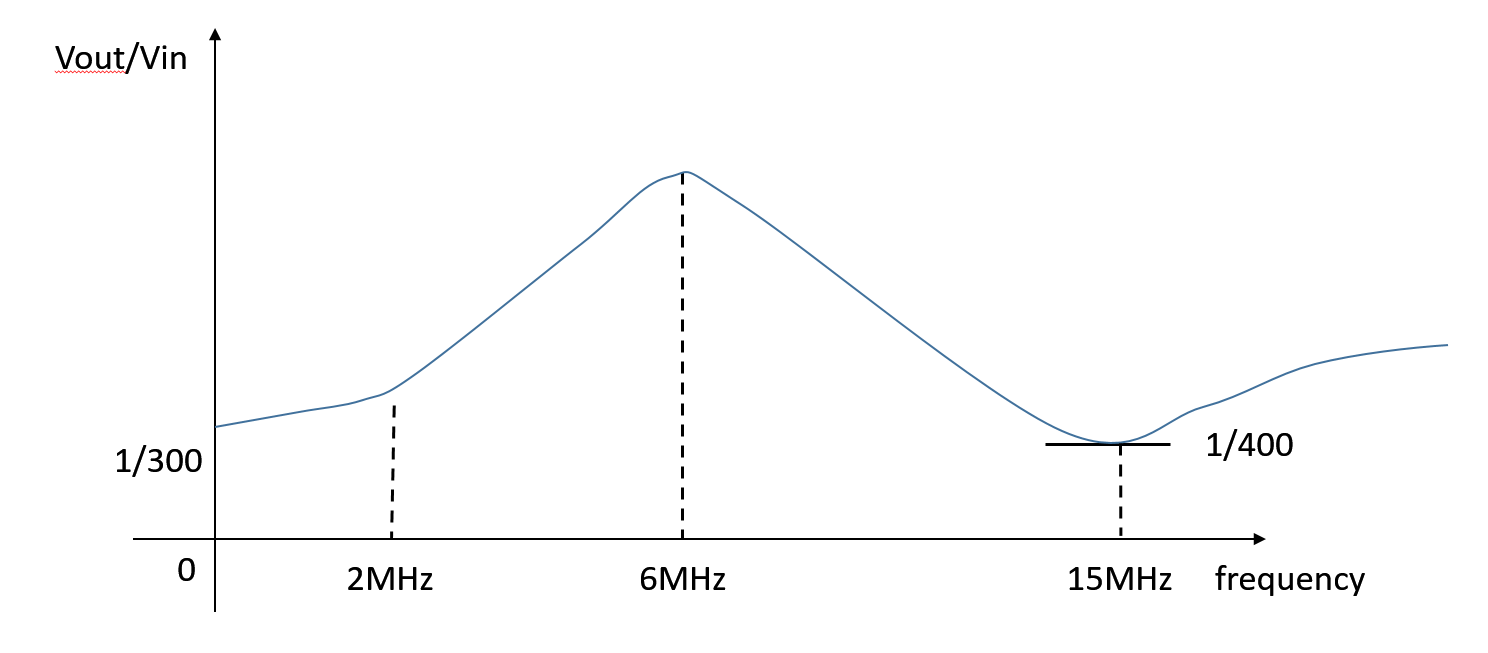
\includegraphics[width=\linewidth/2]{act4}
  \caption{The $V_{out}/V_{in} - frequency$ plot for a difference amplifier}
  \label{fig:act4}
 \end{center}
\end{figure}


\begin{figure}[H]
 \begin{center}
  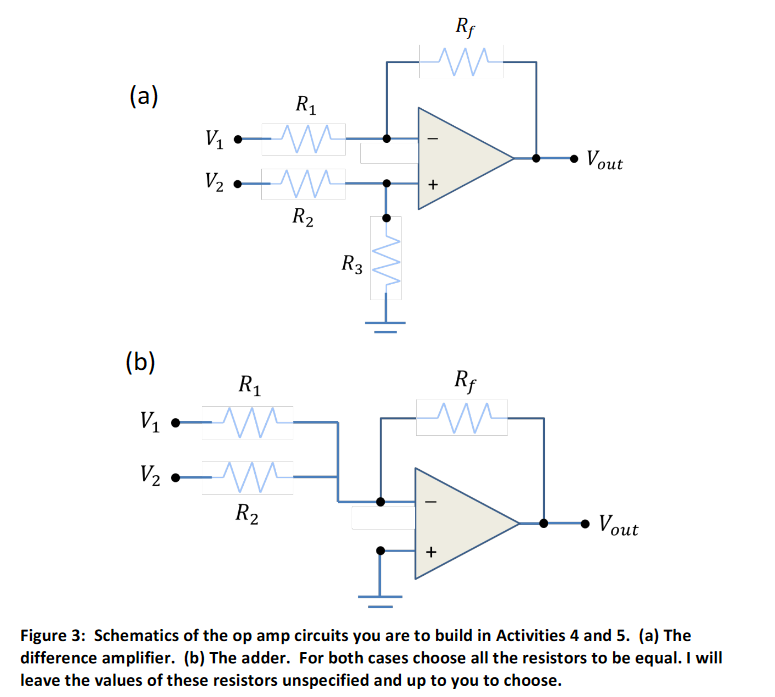
\includegraphics[width=\linewidth/1]{act4and5}
  \caption{}
  \label{fig:act4and5}
 \end{center}
\end{figure}

\section{Activity V - The Op-Amp Adder}

\begin{figure}[H]
 \begin{center}
  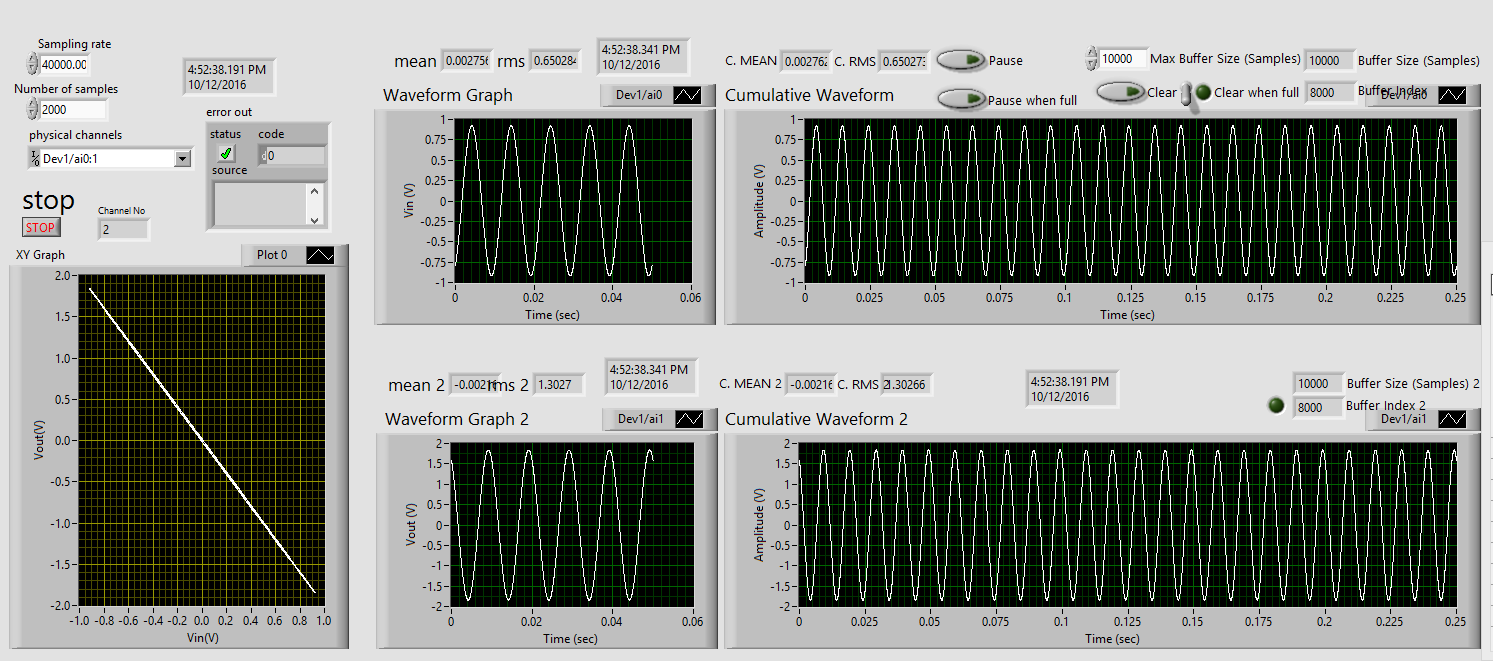
\includegraphics[width=\linewidth/1]{act5AC_V1eqV2}
  \caption{The front panel the VI when $V_{1}=V_{2}$}
  \label{fig:act5AC_V1eqV2}
 \end{center}
\end{figure}

As shown in the picture above, we set $V_{2}=V_{1}=V_{in}$, so you can see that in our plot $V_{out}=-(V_{2}+V_{1})=2V_{in}$, which is consistent with what we expect. And the following shows the derivation of the operation of the ideal adder amplifier.

As shown is figure 8,

$I_{f}=I_{1}+I_{2}=-({V_{1}\over R_{1}}+{V_{2}\over R_{2}})$

$R_{1}=R_{2}=R_{f}$

Inverting Equation: $V_{out}=-{R_{f}\over R_{in}}*V_{in}$

so, $V_{out}=-({R_{f}\over R_{1}}V_{1}+{R_{f}\over R_{2}}V_{2})=-(V_{1}+V_{2})$

The following picture shows what we observed for an op-amp adder.

\begin{figure}[H]
 \begin{center}
  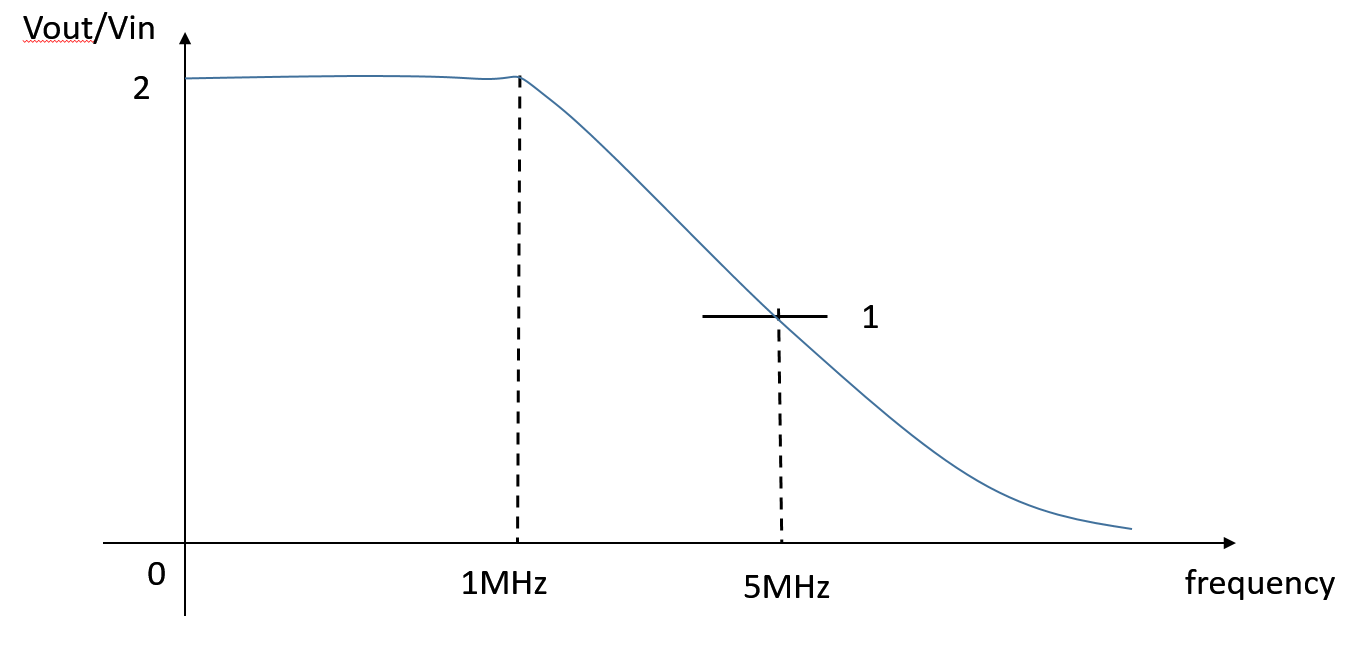
\includegraphics[width=\linewidth/2]{act5}
  \caption{The $V_{out}/V_{in} - frequency$ plot for a op-amp adder}
  \label{fig:act5}
 \end{center}
\end{figure}

\section{Activity VI and VII - The Differentiator and the Integrator}

\begin{figure}[H]
 \begin{center}
  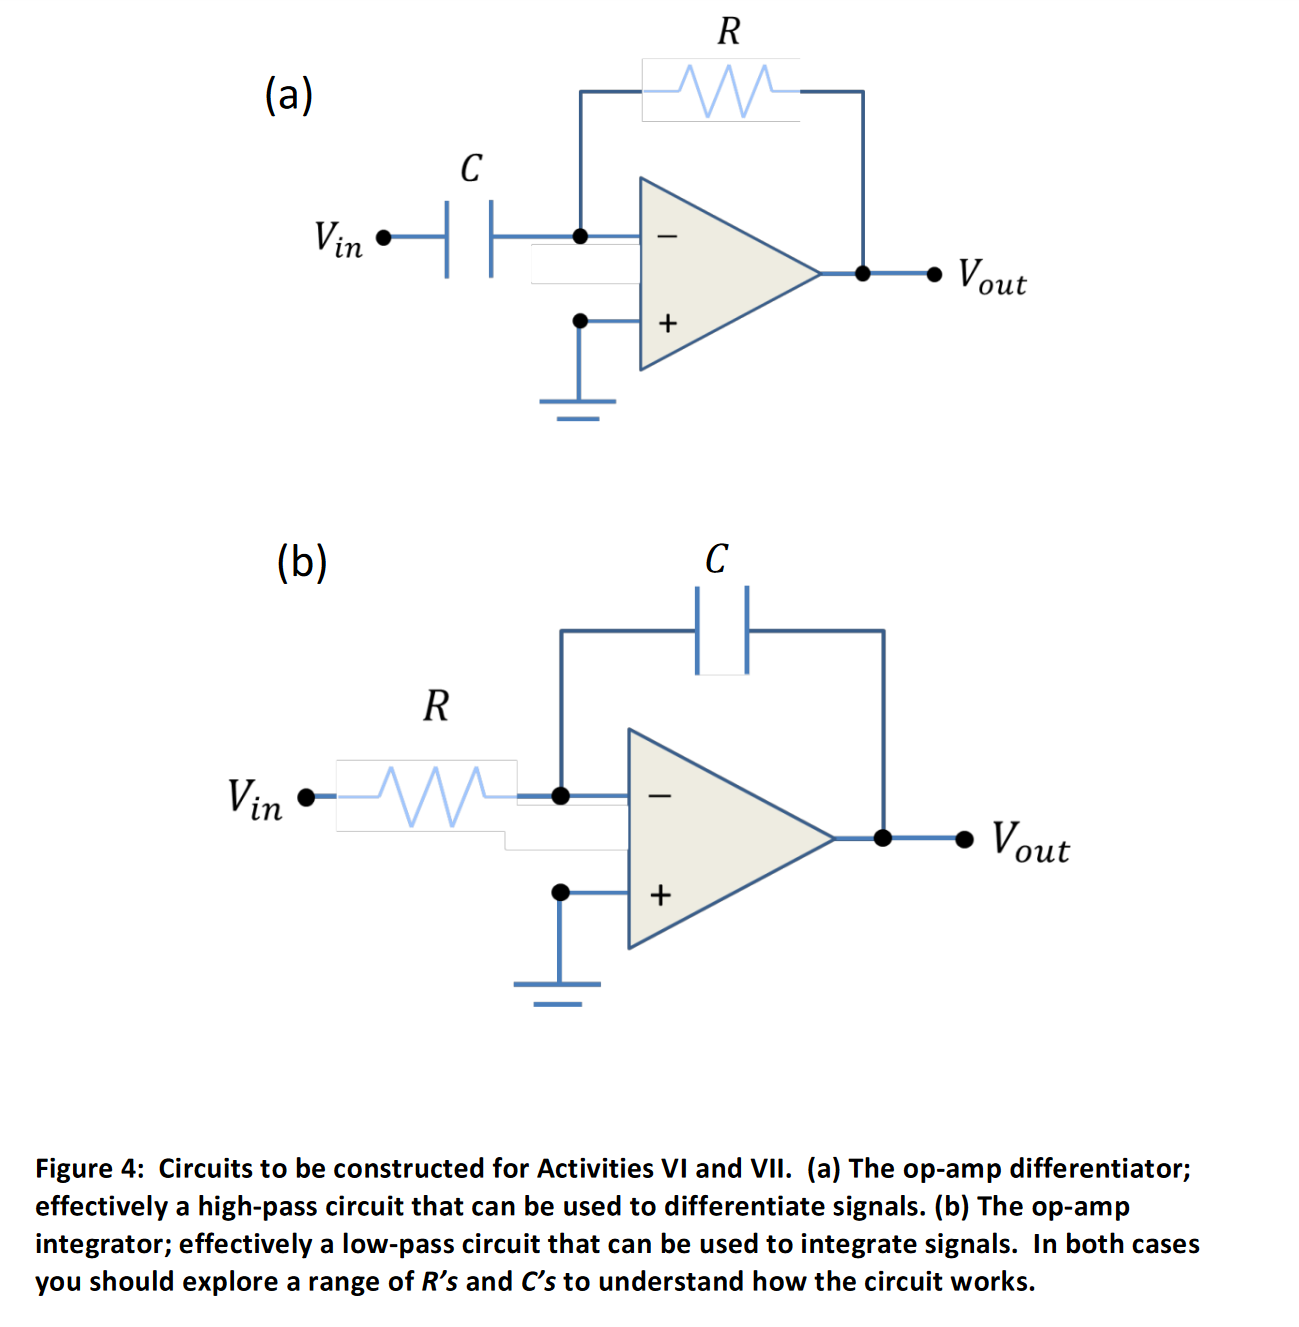
\includegraphics[width=\linewidth/1]{act6and7}
  \caption{}
  \label{fig:act6and7}
 \end{center}
\end{figure}

For an Op-Amp differentiator:

The golden rule $\Rightarrow I_{-}=0$ and $V_{-}=V_{+}=0$

$\Rightarrow I_{in}=I_{R}$

and $I_{R}=-{V_{out}\over R}$

$Q=C*V_{in}$

$\Rightarrow {dQ\over dt}=C{dV_{in}\over dt}$

$I_{in}=C{dV_{in}\over dt}=I_{R}$

$\Rightarrow -{V_{out}\over R}=C{dV_{in}\over dt}$

$\Rightarrow V_{out}=-RC{dV_{in}\over dt}$

\vbox{}

For an Op-Amp integrator:

The golden rule $\Rightarrow I_{-}=0$ and $V_{-}=V_{+}=0$

$\Rightarrow V_{C}=V_{-}-V_{out}=0-V_{out}=-V_{out}$

$V_{C}={Q \over C}$

$\Rightarrow -{dV_{out} \over dt}={dQ \over Cdt}={1 \over C}{dQ \over dt}$

$I_{in}={{V_{in}-0}\over R}={V_{in}\over R}$

$I_{C}=C{dV_{out} \over dt}=C{dQ \over Cdt}={dQ\over dt}={dV_{out}C \over dt}$

$\Rightarrow I_{in}=I_{C}=C{V_{in} \over R}={dV_{out}C \over dt}$

$\Rightarrow {V_{in}\over V_{out}}*{dt\over R_{in}C}=1$

$\Rightarrow V_{out}=-{1\over R_{in}C}\int_{0}^{t}V_{in}dt=-\int_{0}^{t}V_{in}{dt\over R_{in}C}$


\begin{figure}[H]
 \begin{center}
  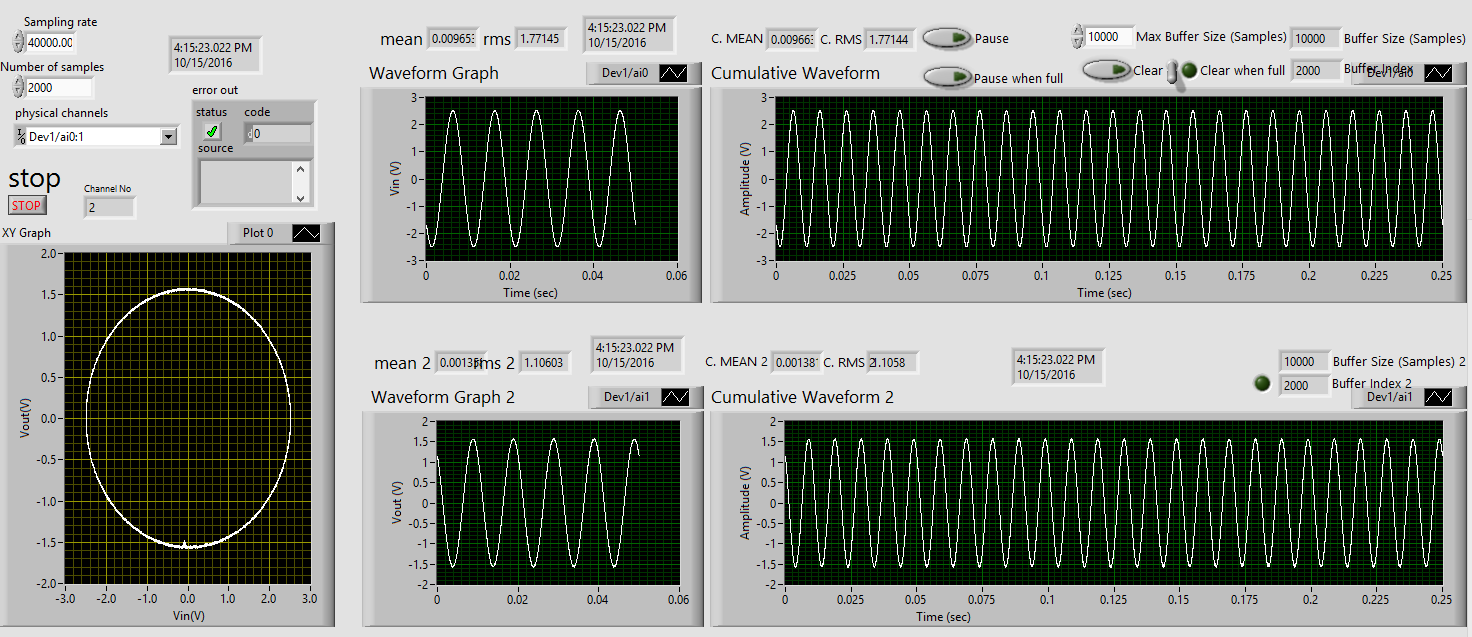
\includegraphics[width=\linewidth/1]{act6diff_sin}
  \caption{The front panel of Op-Amp differentiator for sine wave}
  \label{fig:act6diff_sin}
 \end{center}
\end{figure}

\begin{figure}[H]
 \begin{center}
  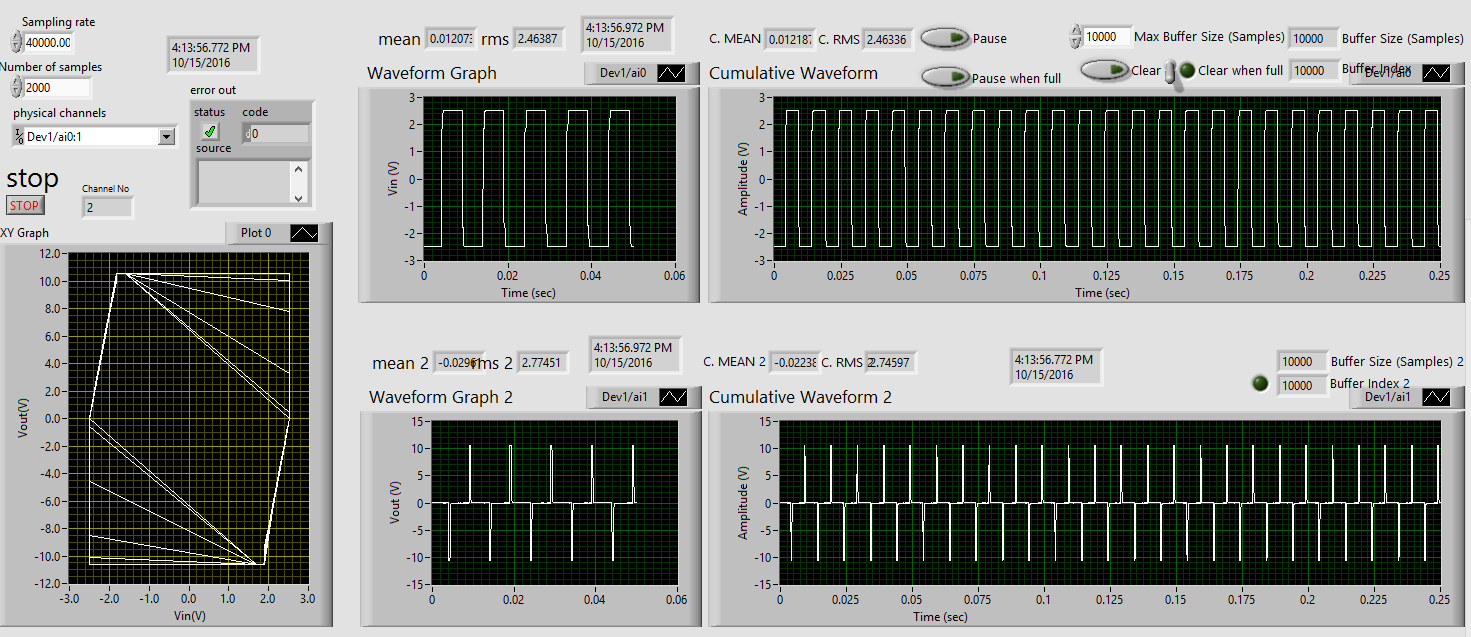
\includegraphics[width=\linewidth/1]{act6diff_square}
  \caption{The front panel of Op-Amp differentiator for square wave}
  \label{fig:act6diff_square}
 \end{center}
\end{figure}

\begin{figure}[H]
 \begin{center}
  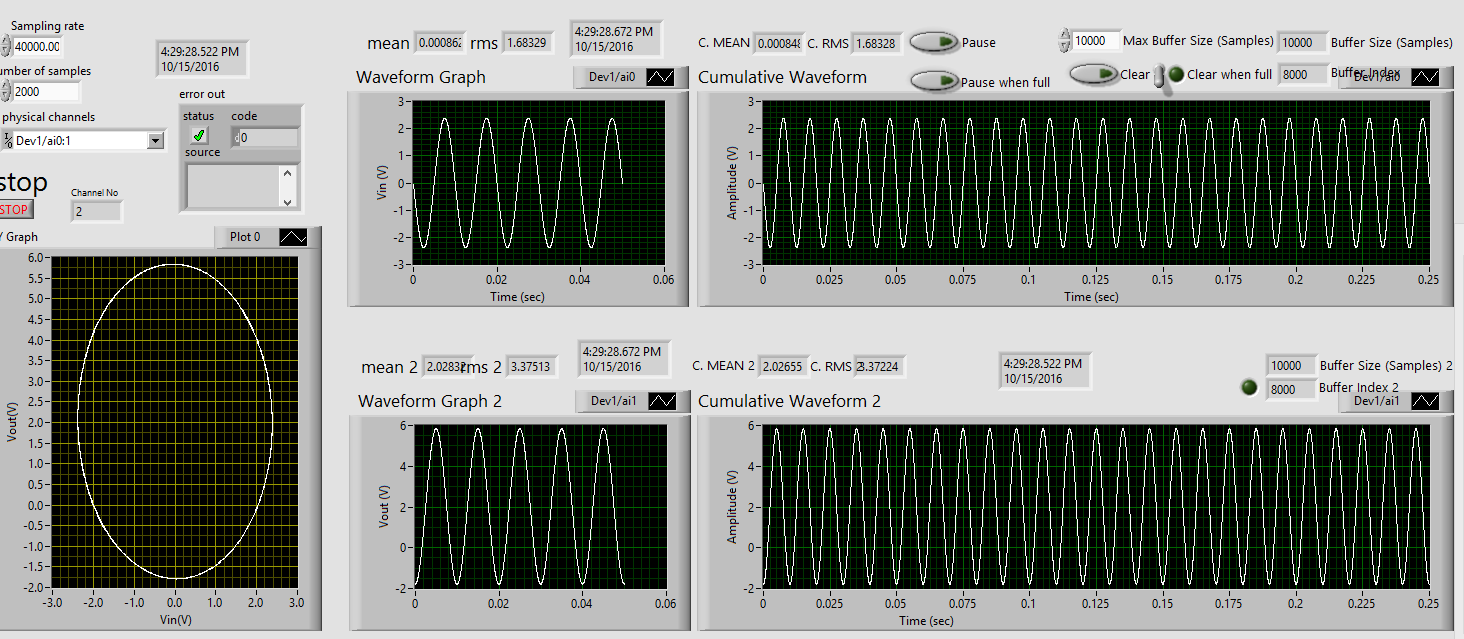
\includegraphics[width=\linewidth/1]{act6inte_sin}
  \caption{The front panel of Op-Amp integrator for sine wave}
  \label{fig:act6inte_sin}
 \end{center}
\end{figure}

\begin{figure}[H]
 \begin{center}
  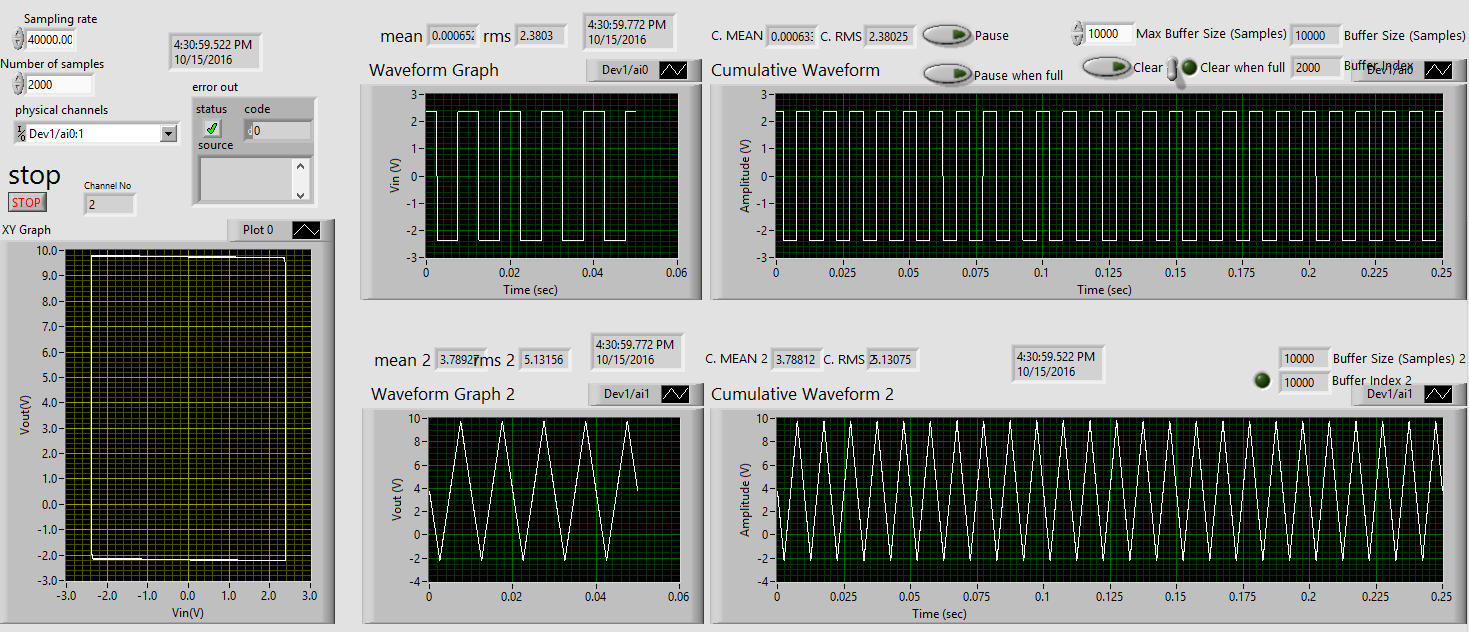
\includegraphics[width=\linewidth/1]{act6inte_square}
  \caption{The front panel of Op-Amp integrator for square wave}
  \label{fig:act6inte_square}
 \end{center}
\end{figure}

Our method to balance the integration circuit is to add a large resistor in parallel with the capacitor, so that the low-frequency signal won't pass the capacitor (will pass the resistor).

\begin{figure}[H]
 \begin{center}
  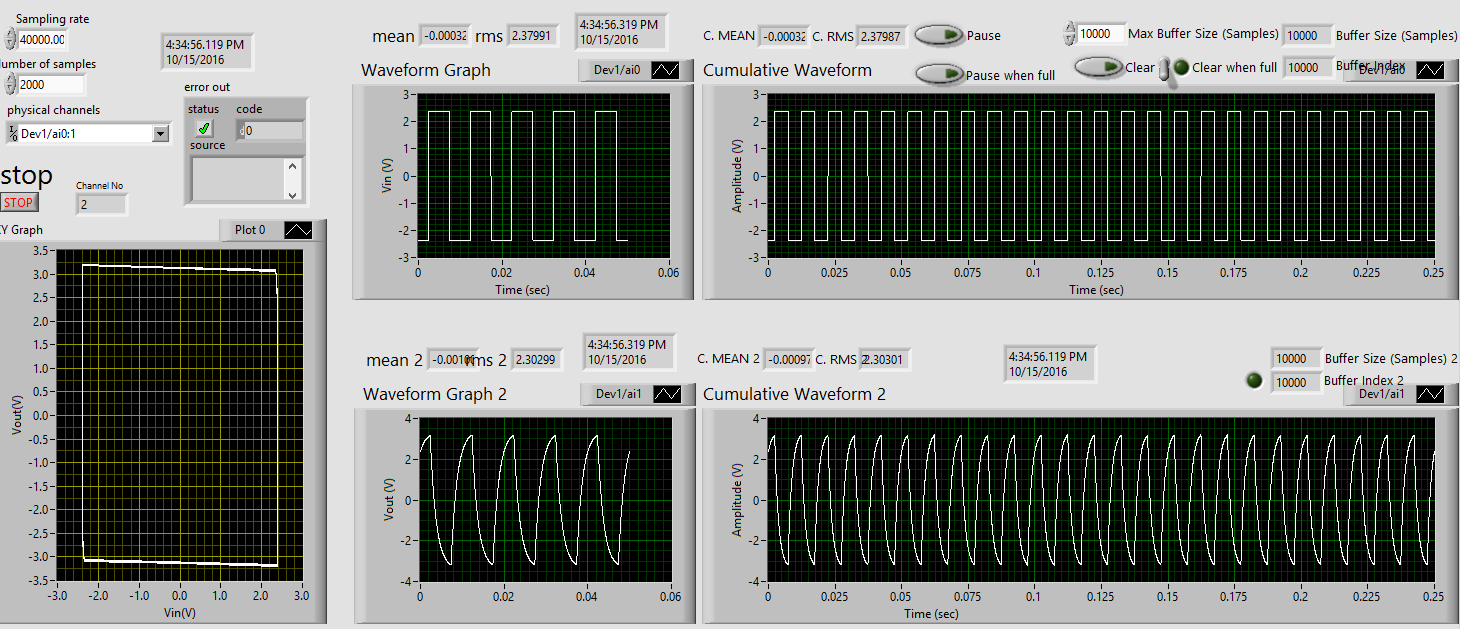
\includegraphics[width=\linewidth/1]{act6inte_square_lowResist}
  \caption{The front panel of Op-Amp integrator for square wave with a resistor}
  \label{fig:act6inte_square_lowResist}
 \end{center}
\end{figure}

\section{Activity VIII - The Transimpedance Amplifier}

\begin{figure}[H]
 \begin{center}
  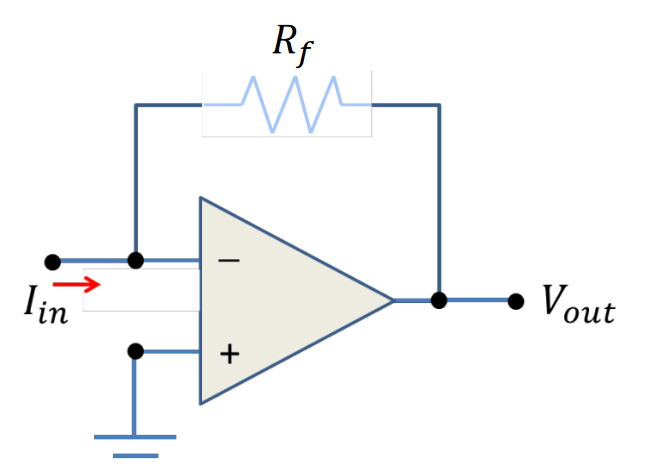
\includegraphics[width=\linewidth/1]{act8b}
  \caption{The Transimpedance Amplifier}
  \label{fig:act8b}
 \end{center}
\end{figure}

The golden rule $\Rightarrow I_{-}=0, V_{-}=V_{+}=0$

$\Rightarrow V_{out}=-I_{in}R_{f}$

This relationship can be usedfor measuring miniscule levels of current.

For this lab, in order to build a current source to supply the current, we added a large resistor $R_{s}$ in series with a voltage source, so $I_{in}={V_{in}\over R_{s}+R_{f}}$. So if we want to measure a very small $I_{in}$, we need to make $R_{s}$ very large. But now we set $R_{s}=R_{f}=1K\Omega $, so in the following figure, $V_{out}=-{R_{f}\over R_{s}}V_{in}=-V_{in}$, which is as same as an inverting amplifier, so all the results can be seen in activity 2.


\end{document}
